\documentclass[11pt]{article}
\usepackage[margin=1in]{geometry}
\usepackage{times}
\usepackage{hyperref}
\usepackage{listings}
\usepackage{xcolor}
\usepackage{booktabs}
\usepackage{amsmath}
\usepackage{graphicx}
\usepackage{caption}

\hypersetup{colorlinks=true, linkcolor=blue, urlcolor=blue, citecolor=blue}
\captionsetup{font=small, labelfont=bf}

\title{TaxBombAI: Open, Auditable Retirement Tax Exposure Projection}
\author{Jitendra Rout \\ \small Independent Researcher \\ \small \texttt{[email/GitHub link]}}
\date{September 2026}

\begin{document}
\maketitle

\begin{abstract}
Retirement tax planning tools that project Required Minimum Distributions
(RMDs) and their associated tax exposure are widely offered by financial
institutions, but are typically closed-source, making their underlying
methodology impossible for an independent party to verify. Separately, a
growing number of financial tools now layer large language model (LLM)
explanations atop computed figures, raising a distinct trust question: does
the generated narrative accurately reflect the numbers it purports to
describe, or does it introduce unverified claims? This paper presents
TaxBombAI, an open-source RMD and tax-exposure projection tool with an
explicit architectural separation between a deterministic calculation
engine and an LLM narration layer, together with three forms of
independent validation: (1) cross-validation of the calculation engine
against an independently re-implemented reference oracle across 500
randomized scenarios (10,318 individual year-level figures), finding
exact agreement within rounding tolerance; (2) a parameter sweep
characterizing how peak RMD magnitude and lifetime tax exposure scale
with starting balance, age, and Roth conversion strategy; and (3) an
automatic faithfulness verifier that checks whether AI-generated
narrative text contains only numeric claims traceable to the underlying
computed schedule, validated against constructed test narratives with
known injected fabrications. We report this as evidence of the
calculation engine's correctness and of a workable verification approach
for AI-narrated financial explanations, while being explicit that the
faithfulness verifier has been validated against constructed test cases
and not yet against live model output, which we identify as the clearest
next step.
\end{abstract}

\section{Introduction}

Required Minimum Distribution (RMD) rules require holders of traditional
tax-deferred retirement accounts to begin withdrawing, and paying tax on,
a portion of their balance from a specified age onward. Because account
balances compound for years before RMDs begin, the resulting tax
liability can be substantial and is frequently larger than account
holders anticipate — informally termed a "tax bomb" in financial
planning discussion. Software tools that project this exposure are
common, offered by financial institutions, advisors, and consumer
finance sites; however, the substantial majority are closed-source,
meaning a user or independent reviewer cannot inspect the underlying
formula, verify it against the source IRS tables, or confirm the tool is
free of implementation error.

A second, more recent trend compounds this opacity concern: financial
tools increasingly layer an LLM-generated natural-language explanation
on top of computed figures, intended to make the output more
accessible to a non-technical user. This introduces a distinct failure
mode beyond a possible calculation bug — the narrative layer could, in
principle, state a figure that does not match what was actually
computed, whether through model error or ungrounded elaboration. To our
knowledge, open financial planning tools that layer AI narration rarely
publish any mechanism for verifying that the generated narrative remains
faithful to the underlying computation.

This paper makes three contributions. First, we describe TaxBombAI's
architecture, which enforces a strict separation between a deterministic
calculation engine and an LLM narration layer instructed to narrate,
not compute, so that the numeric output remains auditable independent of
the AI layer. Second, we validate the calculation engine through
independent cross-implementation: a from-scratch re-implementation of
the RMD projection formula in a different language, checked against the
production implementation across 500 randomized scenarios. Third, we
introduce and validate an automatic faithfulness verifier — a non-AI,
pattern-based checker that flags numeric claims in AI-generated
narrative text unsupported by the underlying computed schedule — and
report its validation against constructed test cases with deliberately
injected fabrications, while being explicit that evaluation against live
model output remains future work.

\section{System Architecture}

TaxBombAI consists of three components. The \textbf{calculation
engine} (\texttt{src/calculator.js}) implements RMD projection using the
IRS Uniform Lifetime Table (Publication 590-B, Table III), a
configurable marginal tax bracket schedule, and a Roth conversion ladder
comparison mode. It is a pure function of its inputs, with no external
dependencies or network calls, making it independently testable and
auditable. The \textbf{narration layer} (\texttt{src/explainer.js})
sends only the already-computed schedule to an LLM (Claude), with an
explicit system instruction not to recompute or invent figures, and asks
it to narrate the result in plain language. The \textbf{faithfulness
verifier} (\texttt{src/faithfulnessVerifier.js}), introduced in this
paper, provides a non-AI, deterministic check of the narration layer's
output: it extracts dollar-figure and age references from generated text
via pattern matching and flags any that do not correspond, within a
small tolerance, to a value actually present in the computed schedule.

This architectural separation is the paper's central design claim: by
construction, the numeric content of TaxBombAI's output does not depend
on the LLM at all, and the LLM's role is strictly narrational. The
faithfulness verifier provides an automatic, auditable check of that
property rather than relying on it as an unverified assumption.

\section{Validation Methodology}

\subsection{Independent Cross-Validation of the Calculation Engine}

We wrote a second, independent implementation of the RMD projection
formula in Python (\texttt{validation/reference\_oracle.py}), transcribing
the IRS Uniform Lifetime Table divisors directly from Publication 590-B
rather than copying the JavaScript implementation's table. We then
generated 500 randomized test scenarios, sampling starting age (45--70),
traditional balance (\$50,000--\$5,000,000), annual growth rate
(0--10\%), RMD start age (73 or 75, per SECURE 2.0), projection horizon
(10--30 years), and other taxable income (\$0--\$150,000) uniformly at
random with a fixed seed for reproducibility. Each scenario was run
through both the production JavaScript calculator and the independent
Python oracle, and every individual year-level output (RMD amount,
taxable income, estimated tax, ending balance) was compared between the
two implementations.

\subsection{Parameter Sweep}

To characterize the calculation engine's behavior across realistic input
ranges, we swept starting age ($\{55,60,65,70\}$) and starting
traditional balance ($\{\$250\text{K}, \$500\text{K}, \$1\text{M},
\$2\text{M}, \$4\text{M}\}$) at fixed 6\% growth, RMD start age 73, and
\$40,000 other taxable income, recording the age and magnitude of peak
annual RMD and cumulative lifetime tax for each combination. We
separately swept the annual Roth conversion amount ($\$0$ to
\$150,000/year) for a fixed profile (age 60, \$1.5M starting balance,
conversion window ages 60--72) to characterize the lifetime-tax effect
of the Roth conversion ladder comparison mode.

\subsection{Faithfulness Verifier Validation}

We constructed two test narratives structurally resembling AI-generated
output: one in which every quoted dollar figure and age reference is
drawn directly from a computed schedule (the "faithful" case), and one
structurally identical narrative in which the peak RMD amount and peak
RMD age were each replaced with a nearby but incorrect invented value
(the "unfaithful" case, simulating a hallucinated or miscalculated
figure). We ran the faithfulness verifier against both and checked
whether it correctly classified each. We emphasize that neither
narrative was generated by a live LLM call for this validation — the
faithful narrative was authored to resemble expected model output, and
the unfaithful narrative was constructed by deliberately injecting
known-incorrect values into it. This validates the verifier's detection
logic; it does not constitute an evaluation of the narration layer's
actual behavior when connected to a live model, which we did not have
API access to perform in this evaluation environment and identify as
the clearest direction for follow-up validation.

\section{Results}

\subsection{Cross-Validation}

Across 500 randomized scenarios, comprising 10,318 individual year-level
output rows, the JavaScript production implementation and the
independently-written Python oracle agreed within a \$1 rounding
tolerance on every compared value (RMD amount, taxable income, estimated
tax, and ending balance) with zero mismatches. Table~\ref{tab:crossval}
summarizes the validation run.

\begin{table}[h]
\centering\small
\caption{Cross-validation summary.}
\label{tab:crossval}
\begin{tabular}{lr}
\toprule
Randomized scenarios & 500 \\
Individual year-rows compared & 10,318 \\
Fields compared per row & 4 \\
Mismatches beyond \$1 tolerance & 0 \\
\bottomrule
\end{tabular}
\end{table}

\subsection{Parameter Sweep Findings}

Figure~\ref{fig:scaling} shows peak annual RMD as a function of starting
balance across four starting ages. Two properties are apparent and
directly follow from the model's structure: peak RMD magnitude scales
linearly with starting balance at fixed age and growth rate (since RMD
is computed as balance divided by an age-indexed divisor, and balance
evolution is a linear recursion in the starting balance), while the
\emph{age} at which the peak occurs is invariant to starting balance,
depending only on the growth rate, RMD start age, and the shape of the
Uniform Lifetime Table divisor sequence. This is a useful sanity property
for reviewing the model's internal consistency: any parameter sweep in
which peak-RMD age varied with balance alone, holding other parameters
fixed, would indicate an implementation error.

\begin{figure}[h]
\centering
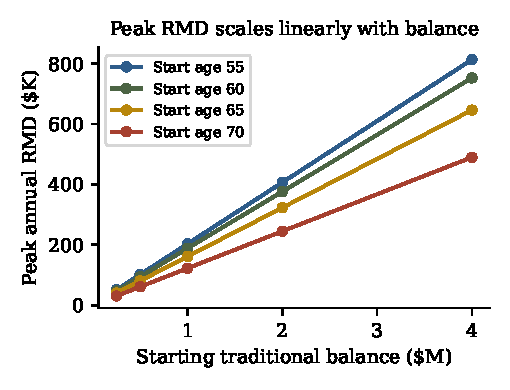
\includegraphics[width=0.7\linewidth]{fig1_peak_rmd_scaling.pdf}
\caption{Peak annual RMD vs.\ starting balance, by starting age (6\% growth, RMD start age 73).}
\label{fig:scaling}
\end{figure}

Figure~\ref{fig:roth} shows lifetime tax savings from the Roth conversion
ladder comparison mode as a function of annual conversion amount, for a
fixed profile (age 60, \$1.5M starting balance). Savings increase with
conversion amount but with clearly diminishing marginal returns
(\$96,238 saved at the first \$25,000/year increment vs.\ \$71,908 saved
at the increment from \$100,000 to \$150,000/year), consistent with the
expected mechanism: early conversions fill lower tax brackets
efficiently, while larger conversions increasingly push into higher
marginal rates, reducing the per-dollar benefit of further conversion.

\begin{figure}[h]
\centering
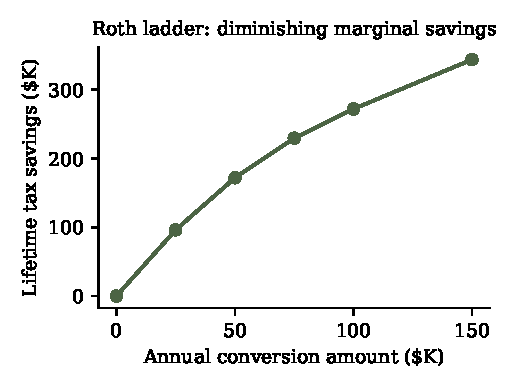
\includegraphics[width=0.7\linewidth]{fig2_roth_savings.pdf}
\caption{Lifetime tax savings vs.\ annual Roth conversion amount (age 60, \$1.5M starting balance, conversion window 60--72).}
\label{fig:roth}
\end{figure}

\subsection{Faithfulness Verifier}

The faithfulness verifier correctly classified both constructed test
cases: the faithful narrative (two dollar figures, two age references,
all drawn from the computed schedule) was correctly flagged as faithful
with zero unsupported values; the unfaithful narrative was correctly
flagged as unfaithful, with the verifier identifying both injected
fabrications (an incorrect dollar figure and an incorrect age reference)
by name. We report this as validation of the verifier's detection logic
under a controlled, known-answer test, not as an evaluation of the
narration layer's real-world behavior.

\section{Discussion}

The cross-validation result (zero mismatches across 10,318 compared
values between two independent implementations) provides meaningfully
stronger evidence of the calculation engine's correctness than testing a
single implementation against its own internal logic would, since a
systematic error shared by both a piece of code and its own unit tests
would not be caught by that approach, whereas an independent
re-implementation written from the source IRS tables directly provides
an external check.

The parameter sweep's structural finding — peak RMD age is invariant to
starting balance while peak RMD magnitude scales linearly with it — is a
useful property for anyone reviewing or extending this codebase: it
provides a simple, checkable invariant that any correct implementation
of this specific model should satisfy, independent of re-running the
full cross-validation suite.

The faithfulness verifier represents, we believe, a reasonable minimum
bar for AI-narrated financial tools: an automatic, non-AI check that
narrated figures are traceable to the underlying computation, rather
than trusting the narration layer's fidelity as an unverified design
assumption. We are explicit, however, that what we have validated here
is the verifier's ability to distinguish constructed faithful and
unfaithful text — a necessary but not sufficient step toward validating
the narration layer's actual behavior in production, which requires
live-model evaluation we did not have the infrastructure to perform in
this work.

\section{Limitations}

\begin{itemize}
\item \textbf{Faithfulness verifier not yet evaluated against live model
output.} As stated above, our validation used constructed test
narratives, not real LLM-generated text. It is possible that real model
output contains failure modes (e.g., correct figures presented with
misleading qualitative framing, or figures that are technically present
in the schedule but selectively misrepresented) that a purely
numeric-matching verifier would not catch. Live-model evaluation, ideally
across many real generations and multiple models, is the clearest next
step.
\item \textbf{Verifier scope.} The current verifier checks dollar
figures and age references only; it does not verify percentage claims,
qualitative characterizations, or causal claims about which strategy is
better, which would require more sophisticated natural language
understanding than pattern matching provides.
\item \textbf{Tax model simplifications.} As documented in the project's
methodology notes, the bundled tax bracket table is illustrative and not
auto-updated for the current tax year, and does not model state tax,
NIIT, the Social Security taxability phase-in, or filing-status
variations. The Roth conversion ladder comparison does not model the
five-year rule, IRMAA thresholds, or sequence-of-returns risk.
\item \textbf{Cross-validation covers the deterministic engine only.}
The 500-scenario cross-validation validates the calculation engine's
correctness; it says nothing about the narration layer's behavior, which
is addressed separately (and only partially, per above) by the
faithfulness verifier.
\end{itemize}

\section{Conclusion}

We presented TaxBombAI, an open-source RMD and tax-exposure projection
tool built around an explicit separation between a deterministic,
independently-validated calculation engine and an LLM narration layer,
together with an automatic faithfulness verifier for checking that
narrated text remains traceable to the underlying computation. Cross-validation
against an independently re-implemented oracle found zero
mismatches across 10,318 compared values, and the faithfulness verifier
correctly distinguished constructed faithful and unfaithful test
narratives. We regard live-model evaluation of the faithfulness verifier
against real narration-layer output as the most valuable direction for
follow-up work, and release all code, validation scripts, and raw
results openly to support that and other extensions.

\section*{Availability}
All code, validation scripts, and raw results described in this paper
are published under the MIT license at
\url{https://github.com/jitendrarout/taxbombai}.

\section*{References}

[1] Internal Revenue Service. \emph{Publication 590-B: Distributions from Individual Retirement Arrangements (IRAs).} \url{https://www.irs.gov/publications/p590b}

[2] U.S. Congress. \emph{SECURE 2.0 Act of 2022.} Required minimum distribution age provisions.

\end{document}
